\chapter{Конструкторская часть}

В этом разделе будут приведены подробные описания алгоритмов, а также схемы алгоритмов, используемых в растеризаторе.

\section{Разработка алгоритма}

Рассмотрим шаги работы предложенного графического конвейера:

\begin{enumerate}[label={\arabic*)}]
	\item фильтрация объектов не входящих в пирамиду видимости (CPU);
	\item асинхронный анализ виртуальной геометрии (GPU);
	\item создание или обновление виртуальных объектов (GPU);
	\item формирование z-буфера (GPU);
	\item отрисовка объекта на растре (GPU);
	\item вывод растра на экран (OpenGL).
\end{enumerate}

Фильтрация объектов (frustum culling) не релевантна тематике работы.
Рассмотрим оставшиеся шаги в отдельности. 
Был использованы фрагменты кода из tinyrenderer \cite{tinyrenderer} и learnopengl \cite{learnopengl}.

\subsection{Фильтрация объектов не входящих в пирамиду видимости}
Сначала определяются объекты, входящие в пирамиду видимости камеры. Это происходит на центральном процессоре. При большом количестве отрисовываемых объектов используется директива parallel\_for (реализации TBB).
Для объекта, входящего в область видимости, происходит диспетчеризация вызова отрисовки (выполняется на видеокарте).

\subsection{Асинхронный анализ виртуальной геометрии}

В этом шаге считается площадь каждой грани отрисовываемой модели (прошедшей фильтрацию по области видимости).
Грани, площадь которых превышает порог, рекурсивно разбиваются на подграни виртуальной геометрии в следующем шаге.
При этом, на данном шаге вычисляется количество виртуальных граней, чтобы заранее выделить необходимый объем видеопамяти при построении геометрии.

Для копирования граней в новую модель используется алгоритм \newline stream\_packing, основанный на алгоритме prescan.

\begin{figure}[ph!]
	\centering
	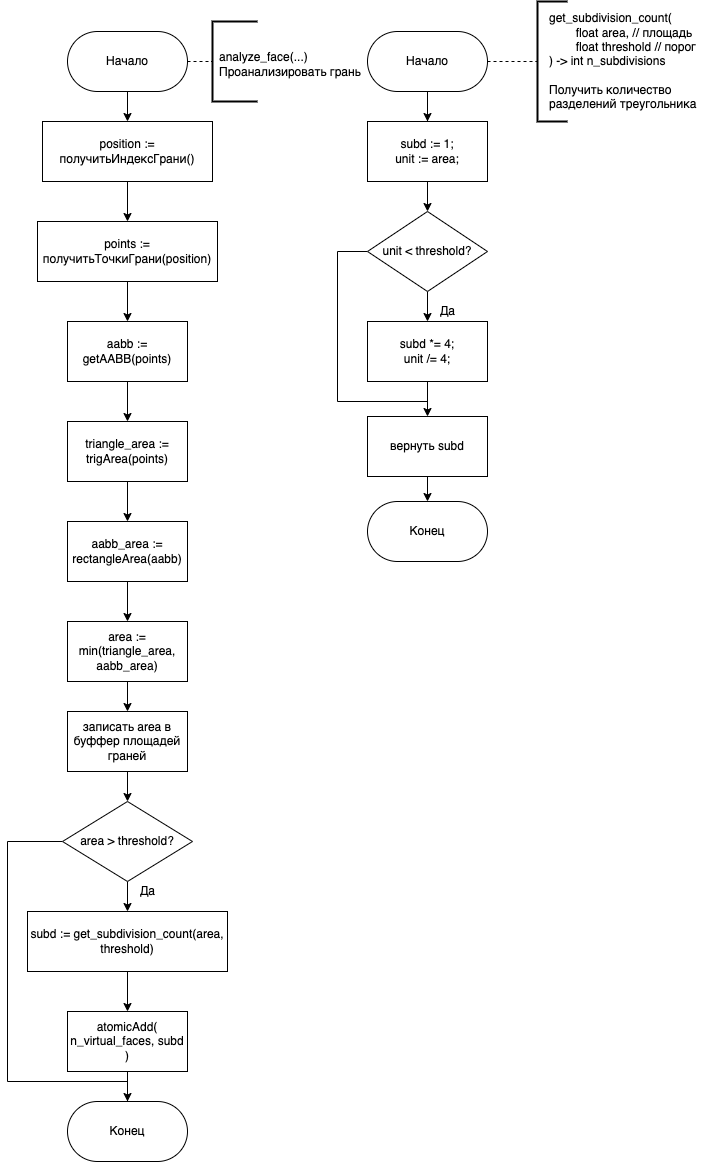
\includegraphics[height=0.95\textheight]{inc/img/diagrams-vgeom_analyzer.drawio.png}
	\caption{Разработка kernel анализа геометрии}
	\label{fig:geom_analyzer_kernel}
\end{figure}

\pagebreak

\subsection{Создание или обновление виртуальных объектов}

Выделяются буферы для вершин, граней и дополнительных векторов нормалей, текстур.

В моей реализации, у меня имеется несколько z-буферов, каждый из которых отвечает за отрисовку одного изображения. В каждом изображении имеется несколько кадров, каждый из которых отвечает за отрисовку группы объектов.

\begin{figure}[ph!]
	\centering
	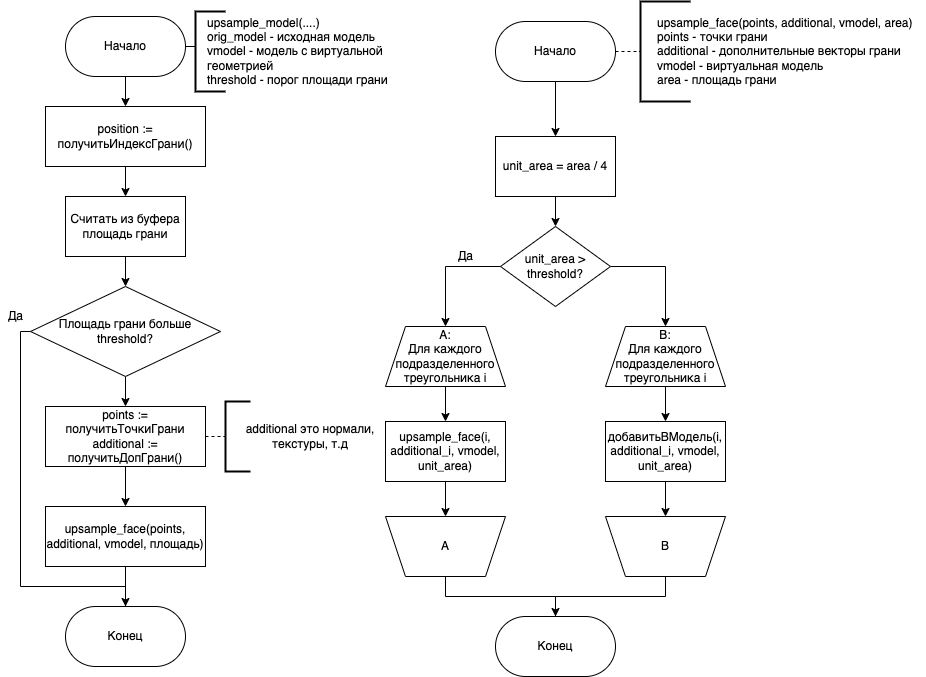
\includegraphics[width=1\linewidth]{inc/img/diagrams-vgeom_upsampler.drawio.png}
	\caption{Разработка kernel создания виртуальной геометрии} 
	\label{fig:vgeom_create_kernel}
\end{figure}

\pagebreak

\subsection{Заполнение z-буфера}

В продложенной реализации используется $ 2^n $ z-буферов, которые заполняются в параллельном режиме.
Группы объектов отправляются в соответствующий z-буфер, используя операцию atomicMax для записи z-значения в разделяемый буфер.

После обработки каждой, происходит слияние z-буферов в один, используя алгоритм параллельной редукции. 
Для параллелизации используется Cuda Stream API.

\begin{figure}[ph!]
	\centering
	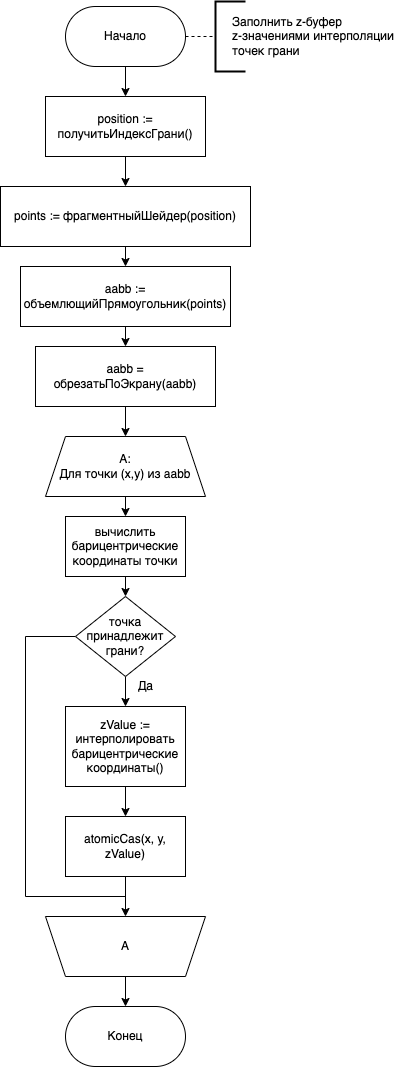
\includegraphics[height=0.95\textheight]{inc/img/diagrams-zfiller.drawio.png}
	\caption{Разработка kernel заполнения z-буфера}
	\label{fig:zfiller_kernel}
\end{figure}

%\begin{figure}[ph!]
%	\centering
%	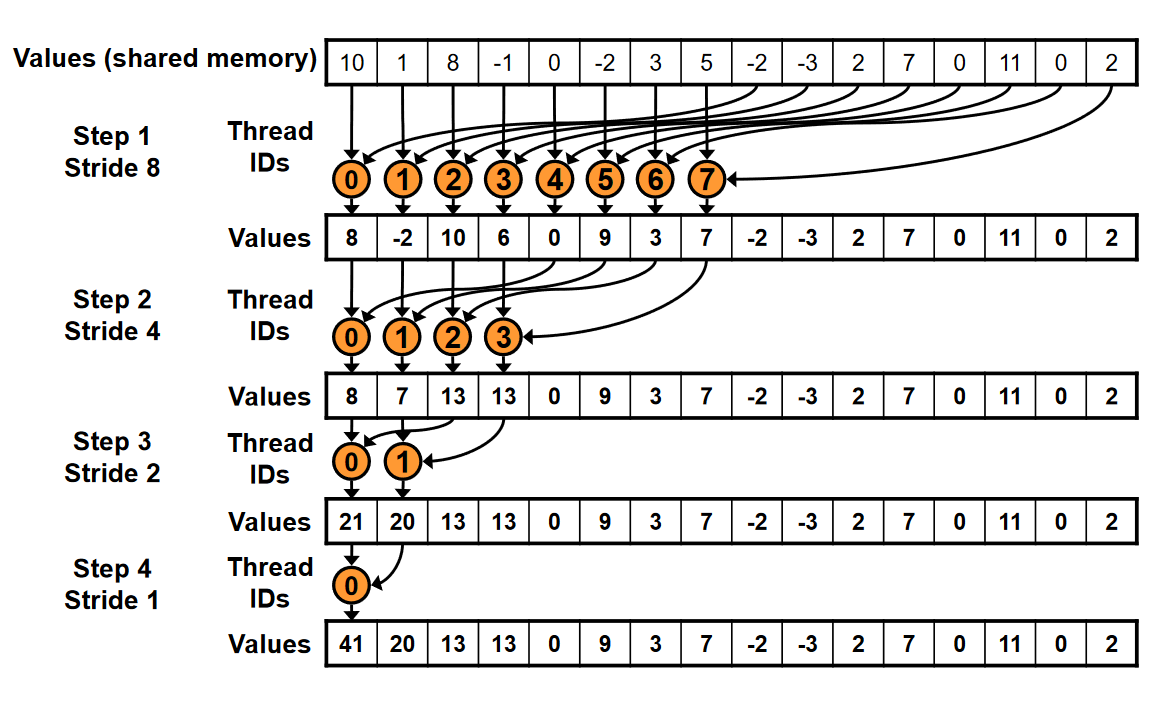
\includegraphics[width=0.95\textwidth]{inc/img/parallel_reduction.png}
%	\caption{Идея работы алгоритма параллельного редуцирования}
%	\label{fig:parallel_reduction_idea}
%\end{figure}

\pagebreak

\subsection{Отрисовка объектов}

После заполнения z-буфера, происходит отрисовка объектов, используя алгоритм растеризации.

Каждая грань отрисовывается в отдельном потоке. Группа объектов сцены отрисовываются в отдельных Cuda Stream.

\begin{figure}[ph!]
	\centering
	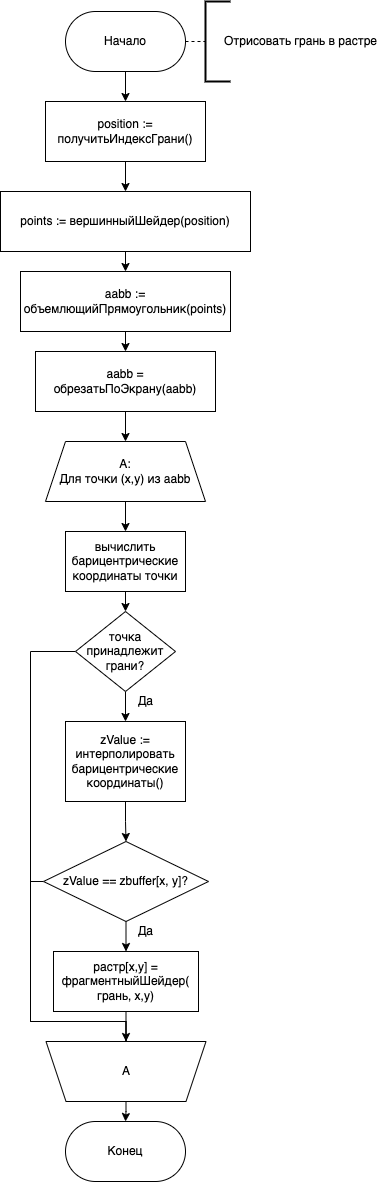
\includegraphics[height=0.95\textheight]{inc/img/diagrams-rasterizer.drawio.png}
	\caption{Разработка kernel растеризации}
	\label{fig:diagram_count}
\end{figure}

\pagebreak

\section*{Вывод}

В ходе выполнения работы разработана и проанализирована система рендеринга, которая позволяет отрисовывать сцены с большим количеством объектов.

Рассмотрены и подробно описаны параллельные алгоритмы, которые позволяют ускорить процесс рендеринга.

